\documentclass[12pt]{article}                  %Mandatory command; select
                                               %   default 10 point type
\usepackage{graphicx} 
\usepackage[colorlinks]{hyperref}
\hypersetup{citecolor=DeepPink4}
\hypersetup{linkcolor=red}
\hypersetup{urlcolor=blue}
\usepackage{cleveref}
					% allows you to insert .jpg files
\usepackage{float}


\setlength{\textheight}{10truein}              % Set height of text area
\setlength{\topmargin}{-0.5truein}             % Center text on 11'' height
\setlength{\textwidth}{6truein}                % Set width of text area
\setlength{\oddsidemargin}{0.25truein}         % Center text on 8.5'' width
\setlength{\parskip}{6pt plus 1pt minus 1pt}   % Specify extra space
                                               %   between paragraphs,
                                               %   allowing LaTeX to adjust
                                               %   space 1 point up or down
\setlength{\parindent}{40pt}                   % Set paragraph indent

\begin{document}                               % Mandatory command

                                               % Large, bold, centered title
\begin{center}
{\large \bf{PHYS 325 Final Project:\\
Programmatic Solutions to the Infinite Square Potential Well}}\\
\end{center}
\begin{flushleft}                              % Two lines; flush left
{\em Author}: A.~J.~Ogle \\                    % \\ forces a new line
{\em Date}: May 10th, 2015\\
{\em PHYS 325 Computational Physics}\\
\end{flushleft}

\section{Introduction}
	The Schrödinger equation describes the motion and energy of quantum particles. It can be used to determine how a system evolves over time, in the case of the time-dependent Schrödinger equation (TDSE). It can also describe the steady state solution for a physical system which does not change over time, in the case of the time-independent Schrödinger equation (TISE). 
	
The TDSE can describe how a particle-wave propagates through space. The TISE can be used for instances in which the wave is stationary, such as a particle trapped in a potential well or box. These "boxes" are simplified representations of actual potential wells, such as the orbitals of an atom. There are instances in which dealing with potentials can be much more complex - so complex that analytic solutions are difficult, if not impossible, to derive. With this in mind, it is important to develop methods which can numerically solve for the wavefunction for any geometry in 2 or 3 dimensions. While this paper will not cover the more advanced methods for solving for the wavefunction of a particle in complicated 3 dimensional potential fields, it will provide a method from which to start. 

\section{Background}

The starting point will be to grapple with solving for the wavefunction in the context of a 1 dimensional infinite square potential well. This situation produces a square potential well because, if applied in the case of 2 dimensions, it produces a  square "well" for the particle to be trapped in. To begin, the 1D TISE must be considered: 

\begin{equation}
\frac{-\hbar}{2m}\frac{d^2\Psi_{x}}{dx^2}+V_{x}\Psi_{x} = E\Psi_{x}
\label{1D TISE}
\end{equation}

Since the potential is infinite at the boundaries, it is assumed that there is zero probability of finding the particle outside the potential barrier. It is also assumed that the wavefunction is continuous across the entire dimension. Since the wavefunction is continuous, the limits approaching the points at the boundary (labeled with $L$, for $L = \frac{+}{-}1$) must exist. From these assumptions, a solution to the wave equation can be solved for which the waves fulfill the boundary conditions. Analytically, it can be found that: 


\pagebreak

\begin{equation}
\Psi_{x} = Acos(\frac{(2n)\pi}{L}x),\: n\: is\: even\: and\: A = \sqrt{\frac{L}{2}}
\label{Wavefunction Solution, even}
\end{equation}
and
\begin{equation}
\Psi_{x} = Asin(\frac{(2n-1)\pi}{L}x),\: n\: is\: odd\: and\: A = \sqrt{\frac{L}{2}}
\label{Wavefunction Solution, odd}
\end{equation}

When solving for stationary wavefunctions numerically, the method of "shooting and matching" will be used. This method assumes an initial value for the energy, then checks whether this energy gives a solution sufficiently close to the boundary conditions ($\Psi_{x} = 0$). If a sufficient solution is not achieved, then the simulation "shoots" again, using a guess for the energy that is either higher or lower by some amount ($dE$), depending on whether the prior guess was too high or too low. This is an algorithm that can also be used for finding the solution to hitting a target in projectile motion, hence the name of "shooting and matching."

To begin, the initial conditions of $\Psi_{0} = 1$ are assumed (this is the point right at the middle of the well) for the case of an even energy level ($n = 0, 2, 4, 6, ...$). This gives a point from which the algorithm can "shoot," using the wave equation and some initial guess for the energy level, to solve for the boundary conditions. In the algorithm, the points of the wave equation can be iterated using: 

\begin{equation}
\Psi_{n+1}= 2*\Psi_{n} - \Psi_{n-1} - 2(\Delta x)^2(E - V_{n})\Psi_{n}
\end{equation} 

The initial conditions for this algorithm are $\Psi_{0} = 1$ and $\frac{d\Psi}{dx} = 0$, which implies $\Psi_{n-1} = 1$ (as used for the first the case of $n = 1$ in the algorithm). 

An initial guess for $E$ is fed to the algorithm, which then solves for the value of the wavefunction across the space until it reaches the boundary. The solution for the boundary is then compared against the boundary condition. For $\Psi_{x\, at\, boundary} > \Psi_{boundary\, condition}$, the guess for $E$ is adjusted by some increment $-dE$, lowering the energy (and hopefully moving $\Psi_{x\, at\, boundary}$ closer to $\Psi_{boundary\, condition}$. If $\Psi_{x\, at\, boundary} < \Psi_{boundary\, condition}$, then $E$ is adjusted by some increment $dE$, moving $\Psi_{x\, at\, boundary}$ higher for the next iteration, and hopefully closer to the boundary condition. For each iteration, the value of $dE$ is halved before multiplied by a directional constant, determined by whether $\Psi_{x\, at\, boundary}$ is higher or lower than the boundary value. 

This process repeats itself until $dE$ has been lowered below some value labeled $dE_{min}$, after which the algorithm stops and the solution is graphed. This is the method of "shooting and matching."

When graphing the solution, symmetry of the wavefunction is assumed in this case, so the solution to the wavefunction is plotted on one side of the x axis, then this solution is "mirrored" and plotted on the opposite side, presenting the proper waveform expected of the stationary solution for a particle-wave in an infinite square potential well. 

\pagebreak

\section{Results}
The aforementioned method of "shooting and matching" was used to determine the values for the first 5 even energy levels ($n = 0, 2, 4, 6, 8$). The results are listed in \ref{wavefunction n = 0}-\ref{wavefunction n = 8}. 

\begin{figure}[H]
\centering
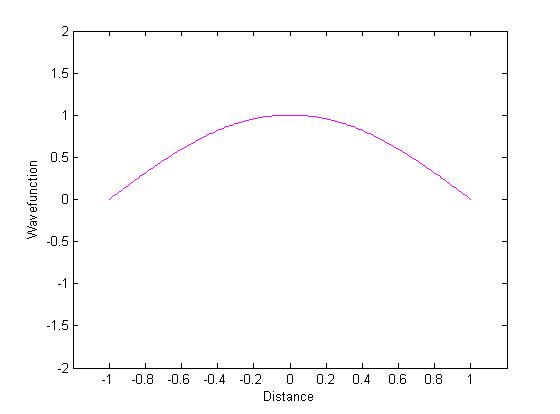
\includegraphics[scale=0.45]{aogle_final_n_0.jpg}
\caption{A solution to the wavefunction for initial energy guess of $E_{0} = 10$. This solution is the $n = 0$ state (ground state), with $E = 1.2715$.}
\label{wavefunction n = 0}
\end{figure}

\begin{figure}[H]
\centering
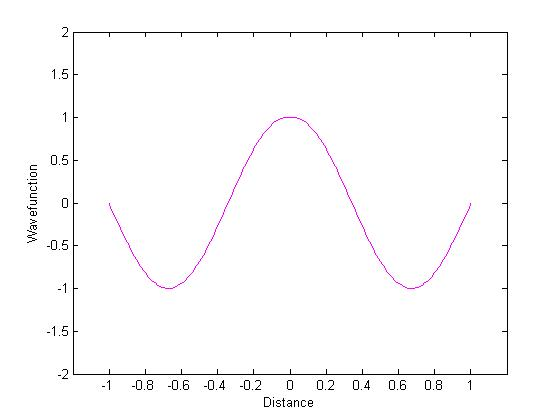
\includegraphics[scale=0.45]{aogle_final_n_2.jpg}
\caption{A solution to the wavefunction for initial energy guess of $E_{0} = 20$. This solution is the $n = 2$ state, with $E = 11.4419$.}
\label{wavefunction n = 2}
\end{figure}

\begin{figure}[H]
\centering
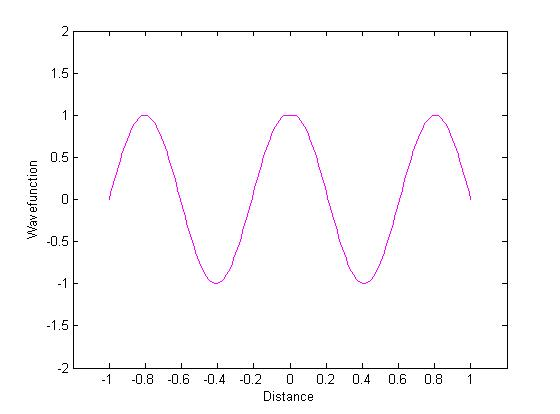
\includegraphics[scale=0.45]{aogle_final_n_4.jpg}
\caption{A solution to the wavefunction for initial energy guess of $E_{0} = 40$. This solution is the $n = 4$ state, with $E = 31.7722$.}
\label{wavefunction n = 4}
\end{figure}

\begin{figure}[H]
\centering
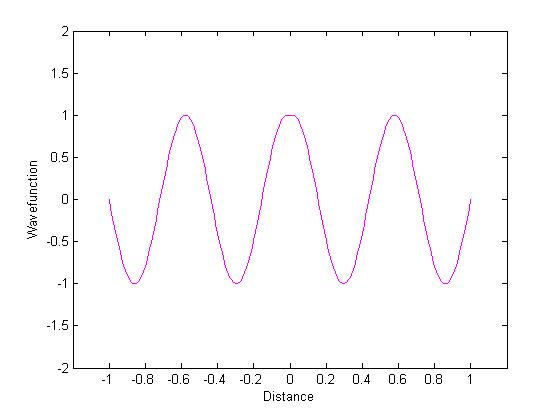
\includegraphics[scale=0.45]{aogle_final_n_6.jpg}
\caption{A solution to the wavefunction for initial energy guess of $E_{0} = 60$. This solution is the $n = 6$ state, with $E = 62.2418$.}
\label{wavefunction n = 6}
\end{figure}

\begin{figure}[H]
\centering
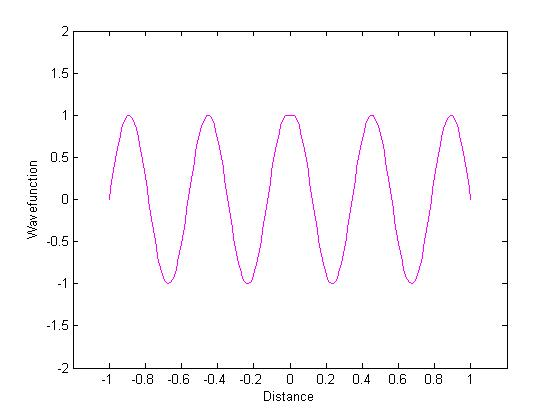
\includegraphics[scale=0.45]{aogle_final_n_8.jpg}
\caption{A solution to the wavefunction for initial energy guess of $E_{0} = 120$. This solution is the $n = 8$ state, with $E = 102.8198$.}
\label{wavefunction n = 8}
\end{figure}

The results from figures \ref{wavefunction n = 0}-\ref{wavefunction n = 8} are summarized in 

\begin{center}
\begin{tabular}{ |c|c|c| }
 \hline
 Energy Level & "Guess" Energy & Solution Energy \\ 
 \hline
 \hline
 n = 0 & E = 10 & E = 1.2715 \\ 
 \hline 
 n = 2 & E = 20 & E = 11.4419 \\ 
 \hline  
 n = 4 & E = 40 & E = 31.7722 \\ 
 \hline
 n = 6 & E = 60 & E = 62.2418 \\  
 \hline
 n = 8 & E = 120 & E = 102.8198 \\ 
 \hline
\end{tabular}
\end{center}

While the energy units are arbitrary (for computational purposes, $-\frac{\hbar^2}{2m} = 1$), the graphs qualitatively match what is expected for the stationary state solutions of the 1D TISE in an infinite square potential well. 


\section{Conclusions}
	Computational methods are a viable way to numerically solve for the wavefunction of particle-waves confined in particular potential wells. For the specific case of an infinite square potential well, the "shooting and matching" method works well due to the symmetry involved. The solutions in this paper were computed with an error of $dE = 0.00001$, an amount which was only limited by the minimal time constraints of an undergrad student equipped with a computer using 8GB of RAM. Solutions with greater amounts of accuracy could viably be found. 
	
For the case of 2 and 3 dimensional solutions, other methods exist. Overall, programmatic solutions to wave equations serve as a powerful tool due to the promising adaptability of the code to any number of initial conditions and geometries. 

\pagebreak
	
One issue with the current code is that the algorithm always searches for the next stable solution at a lower energy level, but not necessarily the solution which is closest to the initial guess. For an initial guess of the energy below the ground state ($E = 1.2715$), the algorithm is unable to find any solution and gets stuck in an infinite while loop. 

A new direction for the program would be to develop a boolean check which would cancel the while loop if an energy below the ground state was found. Another direction would be to develop the program to solve for the odd energy levels. The methods for this solution would be similar, but would rely on using the "shoot and match" method on a different set of initial conditions and utilizing symmetry to plot the wavefunction properly. The case where the potential barrier is not infinite could also be explored. Optimally, the program would model tunneling and the propagation of the wave through a finite barrier with finite potential. 


\begin{thebibliography}{9}

\bibitem{Giordano06}
Giordano, Nicholas J., and Hisao Nakanishi. "10. Quantum" Computational Physics. Upper Saddle River, NJ: Pearson/Prentice Hall, 2006. N. pag. Print.


\end{thebibliography}

\pagebreak
\section{MATLAB code}
\begin{verbatim}
%%Chapter 10.2: One Dimension - Shooting and Matching Methods
clear all;

%Initialize video object
writerObj = VideoWriter('waves_1.avi');
open(writerObj);

prompt = {'Initial Energy Guess:','minimum dE:','speed (<1)'};
dlg_title = 'Input';
num_lines = 1;
def = {'10','0.00001','0.1'};
input = inputdlg(prompt,dlg_title,num_lines,def)';

V_max = 1000;

N = 100; %number of the spatial grids
dx = 0.01; %size of the spatial grids
x = (dx:dx:N*dx);
speed = str2double(input(3)); %the "speed" at which the dE value alters the speed of the movie.

%Initial guess for the increment dE
color = 'm';
E = str2double(input(1));
dE = speed*E;
min_dE = str2double(input(2));
%cutoff parameter
b = 1.5;
keep_going = true;

%Wave Amplitude
L = (0.5*length(x)*dx);
A = L^(-0.5);

%colors for graphing
c = ['r','g','b','y','m','k'];

%Generate the potential for the "infinite" potential well
V = zeros(1,length(x));
V(1) = V_max;
V(length(x)) = V_max;

%Settings for an even parity solution

last_diverge = 0;

%Find the solutions for even energy levels

while (abs(dE) > min_dE && keep_going);

%initial conditions    
Psi_x(1) = 1;
Psi_x(2) = 1;

%calculate the wave equation

    for j = 2:N-1
   
%     if(mod(n,2) == 0)    
%     k = ((n*pi)/L);
%     Psi_x(j) = A*sin(k*x(j));
%     end
%     if(mod(n,2) == 1)
%     k = (((2*n-1)*pi)/(2*L));
%     Psi_x(j) = A*cos(k*x(j));
%     end

    Psi_x(j+1) = 2*Psi_x(j) - Psi_x(j-1) - 2*(E-V(j))*(dx^2)*Psi_x(j);
    
        if(abs(Psi_x(j+1)) > b);
            %assume P_x is diverging
            j = (N);
        end
     
    end

%now we need to mirror the shooting solution for the wave to the other side
%as well
Psi_x_right = Psi_x;
for i = 1:length(Psi_x)
    x_left(i) = -(x(end+1-i));
    Psi_x_left(i) = Psi_x_right(end+1-i);
end
%Then we put it into a single array
Psi_x_total = [Psi_x_left, Psi_x_right];
x_total = [x_left, x];
   
plot(x_total,Psi_x_total,color);
xlabel('Distance')
ylabel('Wavefunction')
axis([-(0.2*N*dx+N*dx) (0.2*N*dx+N*dx) -2 2]);
F(j) = getframe;
writeVideo(writerObj,F(j));


%ask the user if they want to continue the simulation

%     prompt = {'Do you like this solution? (1 - yes, 0 - no)'};
%     dlg_title = 'Input';
%     num_lines = 1;
%     def = {'0'};
%     prompt_ans = inputdlg(prompt,dlg_title,num_lines,def)';
%     
%     x_input = str2double(prompt_ans);
%     if(x_input == 1)
%         keep_going = false;
%     end
%     if(x_input == 0)
%         keep_going = true;
%     end

    if(sign(Psi_x(end))~=sign(last_diverge));
    dE = -0.5*dE; 
    end
    E = E + dE;
    last_diverge = sign(Psi_x(end));
    disp(dE);
    
end
close(writerObj);

disp(E);

\end{verbatim}

\end{document}                                 % Mandatory command
